\section{Kalman Filter Design}
\label{sec:kfdesign}

\subsection{The \acl{KF}}

\nomenclature{$\boldsymbol\Phi$}{State transition matrix of a discrete linear dynamic system}
\nomenclature{$\mathbf G$}{Input matrix}
\nomenclature{$\mathbf H$}{Measurement sensitivity matrix defining the linear relationship between the state of the dynamic system and the measurements that can be made}
\nomenclature{$\mathbf K$}{Kalman gain matrix}
\nomenclature{$\mathbf u$}{Input vector}
\nomenclature{$\mathbf x$}{State vector of a linear dynamic system}
\nomenclature{$\hat{\mathbf{x}}$}{Estimated state vector}
\nomenclature{$\mathbf{z}$}{Measurement vector}
\nomenclature{$\mathbf{w}$}{Process noise vector}
\nomenclature{$\mathbf{v}$}{Measurement noise vector}
\nomenclature{$\mathbf R$}{Covariance matrix of observational (measurement) uncertainty}
\nomenclature{$\mathbf P$}{Covariance matrix of state estimation uncertainty}
\nomenclature{$\mathbf Q$}{Covariance matrix of process noise in the system state dynamics}

A \ac{KF} is used as a type of observer that can be applied to estimate the state vector. This is done to filter the measurements from the vessel and smooth these. If the measurements are too noisy, such that the vessel changes direction suddenly, but should be surging forward, a filter can predict the modelled direction and compare this to the measurement and apply a more correct measurement for the system.

The \ac{KF} comprises the deterministic part, the measurement noise, of the model, which estimates the state vector. This is corrected by means of measurements to estimate the final state vector.

The \ac{KF} is drawn as a block diagram as seen on figure~\vref{fig:blockkf} illustrating both the process and the \ac{KF} together. The upper part represent the process, which can both be a simulated model or the real vessel with measurements, here it is a linear state space model. The lower part is the \ac{KF} which takes in the measurements and estimates the new state vector based on these measurements. The \ac{KF} can be of different types: \ac{LKF}, \ac{EKF} or \ac{UKF}. The figure illustrates the \ac{LKF}. Choosing between these types of filters depends on the type of model used and the application. 

\subsection{\acl{LKF}}
The process model is the usual state space model in discrete form as:
\begin{align}
x_k &= \Phi_{k-1} x_{k-1} + G u_{k-1} + w_{k-1}\\
z_k &= H_k x_k + v_k
\end{align}
\noindent The \ac{LKF} prediction and update can be written as:
\begin{itemize}\tightlist
\item Prediction
\begin{align}
\hat x_k^- &= \Phi_{k-1}\ \hat x_{k-1}^+ + G u_{k-1} \\
P_k^- &= \Phi_{k-1}P_{k-1}^+ \Phi_{k-1}^\top + Q_{k-1}
\end{align}
\item Update
\begin{align}
\bar{\mathbf{z}}_k &= z_k - H_k\ \hat x_k^-\\
S_k &= H_k\ P_k^-H_k^\top + R_k\\
K_k &= P_k^-H_k^\top S_k^{-1}\\
\hat x_k^+ &= x_k^- + K_k \bar{\mathbf{z}}_k\\
P_k^+ &= (I - K_k H_k) P_k^-
\end{align}
\end{itemize}

\begin{figure}
	\centering
	\includesvg{kf_on_sys}
	\caption{Block diagram of a \acl{LKF} resulting in the state estimate $\hat x_k^+$.}
	\label{fig:blockkf}
\end{figure}

Where $P_{k}^-$ is the covariance propagation, $P_{k}^+$ is the update of covariance propagation, $Q$ is a covariance matrix with sensor variances and $R$ is a covariance matrix with model variances. $Q$ is a measure of how much the model is to be trusted. If the variance of the sensors are high this will imply that the model are to be trusted more than the noisy sensor measurements. These variances can sometimes be measured directly at the sensors and used in the $Q$ matrix. This leaves the $R$ matrix as the only design matrix left. $R$ is a measure of how much the measurement are to be trusted. If the variance of the model are high it might be better to trust the actual measurements. $z_k$ is the measurements from the sensors and $\bar{\mathbf{z}}_k$ is the difference between the measurements and the predicted state vector, $\hat x_k^-$. $S_k$ is the covariance matrix of the residual with the variance of the model included. $K_k$ is the optimal Kalman gain, in a \ac{MMSE} sense. 

\subsection{\acl{EKF}}
The above mentioned \ac{LKF} can only be applied on linear systems and transitions. Therefore is this not suited at the AAUSHIP. The position from the \ac{GPS} and the acceleration measurements needs to be rotated with a rotational matrix, which leads to non-linearities in the system. This can be seen on figure \vref{fig:intermediate-calc}. This entails that a \ac{LKF} cannot be used and an \ac{EKF} can be suited. The \ac{EKF} is used to linearise the non-linear terms in the system around the current estimate. In this case it will linearise the transition around the current measurements from the sensors to estimate the true output. The \ac{EKF} can be formulated in discrete form with the prediction and an update as:
\begin{itemize}\tightlist
\item Prediction
\begin{align}
\hat x_k^- &= f(\hat x_{k-1}^-,u_{k-1})\\
P_k^- &= F_{k-1}P_{k-1}^+F_{k-1}^\top+Q_{k-1}
\end{align}
\item Update
\begin{align}
\bar{\mathbf{z}}_k &= z_k - h(\hat x_k^-)\\
S_k &= H_k\ P_k^-H_k^\top + R_k\\
K_k &= P_k^-H_k^\top S_k^{-1}\\
\hat x_k^+ &= x_k^- + K_k \bar{\mathbf{z}}_k\\
P_k^+ &= (I - K_k H_k) P_k^-
\end{align}
\end{itemize}
where the state transition and observation matrices are defined by their respective Jacobians:
\begin{align}
F_{k-1} &= \left.\frac{\partial f}{\partial x}\right|_{\hat x_{k-1}^-,u_{k-1}} \label{eq:EKFF}\\
H_k &= \left.\frac{\partial h}{\partial x}\right|_{\hat x_{k}^-}
\end{align}

\subsection{\acl{KF} in the Case of AAUSHIP}
\label{sec:kfonaauship}
The input is given by the forces applied to the vessel. On AAUSHIP with the two twin propellers and two side thrusters as illustrated in section~\vref{sec:thrust_allocation}, this will result in forces in the surge and sway direction as well as a torque around yaw, the roll and pitch torques are neglected, such that the input vector $u_k$ becomes.
\begin{align}
u_k = \tau_k =
\begin{bmatrix}
X & Y & 0 & 0 & N
\end{bmatrix}^\top
\end{align}
These are the forces that can be applied by the thrusters mounted at the vessel. It should be noted that the pitch and roll are not set as input, since no thrusters can control these, and should be treated as model variations.

The discrete input matrix $\Gamma$ is a $17 \times 5$ matrix from the discretised $B$ matrix from equation~\vref{eq:ss}.
% \todo{Should we use $\Gamma$ for $G$ as in done in other sources (e.g. fossen), such that the input matrix is not confused with the restoring force matrix from fossen?}
The $\Gamma$ matrix takes the forces in $X$, $Y$ and $N$ as input, and neglects inputs in $\phi$ and $\theta$. The forces in $\phi$ and $\theta$ are outputs from the system that makes the vessel change in pitch and roll but are not used as inputs. It is not possible to apply a direct force in pitch and roll. It is possible to apply a roll force by actuating the bow thrusters at the same time, but this will mainly result in a sway force. The same goes for the pitch force, where both main thrusters can be actuated and result in a pitch force, but this will mainly result in a surge force. Therefore are these seen as a result of using the surge and sway, and only a output of the system.

The discrete system $\boldsymbol \Phi$ is a $17 \times 17$ from the discretised $A$ matrix from equation~\vref{eq:ss}, but expanded to contain the full state vector calculations.

The dimensions of the different matrices used are checked as a type of sanity check and verify that the matrices are in correct size.

The covariance propagation matrix, the uncertainty of the estimated state, is given by:
\begin{align}
P_k^- &= F_k\ P_{k-1}^-F^\top + Q_k\\
\text{dim}(P_k^-) &= [17 \times 17]\cdot [17 \times 17]\cdot [17 \times 17]^\top + [17 \times 17]
\end{align}
The $Q$ is the variances of each of the states from the full state vector.

The posteriori error covariance matrix, the update, is given by:
\begin{align}
P_k^+ &= (I - K_k\ H_k)P_k^-\\
\text{dim}(P_k^+) &= ([17 \times 17] - [17 \times 7]\cdot [7 \times 17])\cdot [17 \times 17]
\end{align}
which is a measure of the estimated accuracy of the state estimate. Adding a middle calculation as the residual covariance:
\begin{align}
S_k &= H\ P\ H^\top + R\\
\text{dim}(S_k) &= [7 \times 17]\cdot [17 \times 17]\cdot [7 \times 17]^\top + [7 \times 7]
\end{align}
The $R$ is variances from the sensors, which makes it sensor noise terms.

The updated Kalman Gain:
\begin{align}
K_k &= P\ H^\top\ S^{-1}\\
\text{dim}(K_k) &= [17 \times 17]\cdot [7 \times 17]^\top\cdot [7 \times 7]^{-1}
\end{align}
witch is optimal in a \ac{MMSE} sense. %\todo{Hvorfor virkede denne ac ikke? Har fjernet den tidtil videre} - Hah, det var slet ikke den som var fejlen.

State vector
\begin{align}
\hat{\mathbf x}=
\begin{bmatrix}
N & E & x_b & y_b & \phi & \theta & \psi & u & v & p & q & r & \dot u & \dot v & \dot p & \dot q & \dot r
\end{bmatrix}^\top
\end{align}

Measurement vector
\begin{align}
\mathbf z=
\begin{bmatrix}
N & E & \psi & u & v & a_x & a_y
\end{bmatrix}^\top
\end{align}

Measurement matrix defining the relationship between the state of the dynamic system and the measurements
\begin{align}
H_k =
\begin{bmatrix}
1 & 0 & 0 & 0 & 0 & 0 & 0 & 0 & 0 & 0 & 0 & 0 & 0 & 0 & 0 & 0 & 0 \\
0 & 1 & 0 & 0 & 0 & 0 & 0 & 0 & 0 & 0 & 0 & 0 & 0 & 0 & 0 & 0 & 0 \\
0 & 0 & 0 & 0 & 0 & 0 & 1 & 0 & 0 & 0 & 0 & 0 & 0 & 0 & 0 & 0 & 0 \\
0 & 0 & 0 & 0 & 0 & 0 & 0 & 1 & 0 & 0 & 0 & 0 & 0 & 0 & 0 & 0 & 0 \\
0 & 0 & 0 & 0 & 0 & 0 & 0 & 0 & 1 & 0 & 0 & 0 & 0 & 0 & 0 & 0 & 0 \\
0 & 0 & 0 & 0 & 0 & 0 & 0 & 0 & 0 & 0 & 0 & 0 & 0 & 1 & 0 & 0 & 0 \\
0 & 0 & 0 & 0 & 0 & 0 & 0 & 0 & 0 & 0 & 0 & 0 & 0 & 0 & 1 & 0 & 0 
\end{bmatrix}
\end{align}

The covariance matrix of observational (measurement) uncertainty $R_k$ is assumed to be uncorrelated with the other states, such that the matrix only becomes the variances, with no covariance elements as:
\begin{align}
&R_k = \diag{\mathbf{v}} =\\ \nonumber
&\diag{^\text{GPS}\sigma_{N}^2,\ ^\text{GPS}\sigma_{E}^2,\ ^\text{GPS}\sigma_{\psi}^2,\ ^\text{GPS}\sigma_{u}^2,\ ^\text{GPS}\sigma_{v}^2,\ ^\text{IMU}\sigma_{a_x}^2,\ ^\text{IMU}\sigma_{a_y}^2}
\end{align}
These variances can be found by letting the AAUSHIP be in steady state. The sensor outputs are read while in steady state to check the variances from these. This will be the variances of the individual sensor measurements thus the variances of the particular measurements. The test finding these variances can be found in appendix \todo{lav appendix og ref til det her}.

The covariance matrix of process noise in the system state dynamics is $Q_k$ and is assumed to be the variances of each individual state:
\begin{align}
&Q_k = \diag{\mathbf{w}} = \\ \nonumber
&\diag{\sigma_{N}^2, \sigma_{E}^2, \sigma_{x_{b}}^2, \sigma_{y_{b}}^2, \sigma_{\phi}^2, \sigma_{\theta}^2, \sigma_{\psi}^2, \sigma_{u}^2, \sigma_{v}^2, \sigma_{p}^2, \sigma_{q}^2, \sigma_{r}^2, \sigma_{\dot u}^2, \sigma_{\dot v}^2, \sigma_{\dot p}^2, \sigma_{\dot q}^2, \sigma_{\dot r}^2}
\end{align}
The variances of the process can be hard to validate since these can include noises as incoming waves and other disturbances from the environment. Therefore is the matrix $Q$ used as a tuning parameter to set the weighting between how much to trust the model and the measurements.
% The variances can be found by making tests of the AAUSHIP. These should be carried out such that only one type of variance is tested at a time. By doing this, and testing around a known mean of the given state, makes it possible to test the variance of that particular state. The $Q$ matrix is a tuning parameter to set the weighting between how much to trust the model and the measurements.
%\todo{What about $\mathbf w$ and $\mathbf v$? How to determine them correctly? Det er vel den måde som du lavede tests på da du fandt tallene til $v$?}

The $\mathbf F$, equation\ref{eq:EKFF} from the previous calculations, are the $[17 \times 17]$ system matrix, referred to as $\Phi$ in discrete case. This system matrix changes over time due the changes in the heading. The change of heading is not a linear transition which makes the system non-linear and therefore needs to be linearised about the given states of the system. Therefore this matrix is used as the system matrix in the \ac{EKF}, which is implemented in the AAUSHIP. $\Phi$ is designed to be
\begin{align}
\Phi = 
  \left[\begin{array}{c|ccc|c}
    I_{2\times 2} & 0_{2\times 5} & R_z (\psi) & 0_{2\times 3} & 0_{2\times 5}\\ \hline
    0_{10\times2}  & \multicolumn{3}{c}{\multirow{1}{*}{{$A_d$}}} \vline&  0_{10\times 5} \\ \hline
    0_{5\times 7} & & A_{d[6:10]} & & I_{5\times 5}
  \end{array}\right]
\end{align}
\todo{fix lower left corner alignment vline}

\subsection{Determination of Observational Uncertainty}
The matrix R represents covariance matrix of observational (measurement) uncertainty. This is the matrix which sets the individual variances of the specific measurements from the sensors, the measurements from the output vector $z$. This means that the coefficients of the R matrix can be determined within some interval. The disturbances of each sensor measurement highly depends on which sensor is implemented in the used system. When looking at the AAUSHIP the sensors are of higher accuracy, which means that the sensors are to some extend trustworthy. There are two types of sensors in the AAUSHIP, one \ac{GPS} and an \ac{IMU}. There are two types of \ac{GPS}s installed; a \ac{RTK} \ac{GPS} and a standard \ac{GPS}. At the moment is only the standard \ac{GPS} used, which estimates having a variance of 3 metres radius in the \ac{NED}-frame \todo{Ret dette til noget emre rigtigt efter en måling mere}. The \ac{IMU} consists of a magnetometer, a gyro and an accelerometer. The magnetometer measurements is not used directly and the variance of this is not needed in the R matrix. The gyro neither used in the R matrix. These are not used as measurements directly and therefore not appears in the R matrix. The accelerometer measurements are used in the x and y directions. These have a measured accuracy of 0.00033 $m/s^2$. The \ac{GPS} have different accuracies dependent on which type is used. The main type used will be the \ac{RTK} \ac{GPS} which has higher accuracy than the standard \ac{GPS}. The resulting R matrix, with the standard \ac{GPS}, is estimated from the measurements of $z$ and determined to be
\begin{align}
&R_k = \diag{\mathbf{v}} =\\ \nonumber
&\diag{^\text{GPS}\sigma_{N}^2,\ ^\text{GPS}\sigma_{E}^2,\ ^\text{GPS}\sigma_{\psi}^2,\ ^\text{GPS}\sigma_{u}^2,\ ^\text{GPS}\sigma_{v}^2,\ ^\text{IMU}\sigma_{a_x}^2,\ ^\text{IMU}\sigma_{a_y}^2}\\ \nonumber
&\diag{3\hspace{3mm} 3\hspace{3mm} 13.6\cdot 10^{-6}\hspace{3mm} 0.2\hspace{3mm} 0.2\hspace{3mm} 0.00033\hspace{3mm} 0.00033}
\end{align}

\subsection{Determination of Process Noise}
The matrix Q represents the covariance matrix of process noise in the system state dynamics. This matrix includes parameters as disturbances in the process itself. When looking at the AAUSHIP this could for instance be the incoming waves acting as disturbances both in the roll, pitch and the heading. These types of disturbances can be hard to measure and put a precise number to. Instead, this matrix is used as a tuning parameter for the \ac{KF}, where it sets a weighting of how much the process, and therefore the model, are to be trusted. If the sensors has a high accuracy, it would be of benefit to trust these more than the process, thus setting the parameter of this specific measurement in the Q matrix high. But the Q matrix is used to combine the measurements and the model prediction together. This means that based on the variances from the Q matrix, based on the values from the R matrix, it is tuned to get the best performance from the combination of the model and the measurements

As the model of the AAUSHIP is made, it becomes possible to tune the parameters of Q in a systematic way. The model decouples the acceleration from the velocity, and the velocity from the position. Therefore it is of benefit to tune the acceleration noise variance firstly, such that this makes a proper fit to a step function. A test can be simulated where the AAUSHIP accelerates to a certain velocity and keeps this velocity. This needs to fit such that it makes the AAUSHIP follow a satisfying curve in each of the acceleration, velocity and position tests. The simulation curve is both based on measurements and model predictions. A wanted acceleration curve, for instance in surge and sway, will look like on figure \ref{fig:uvacceltest}.
\begin{figure}
  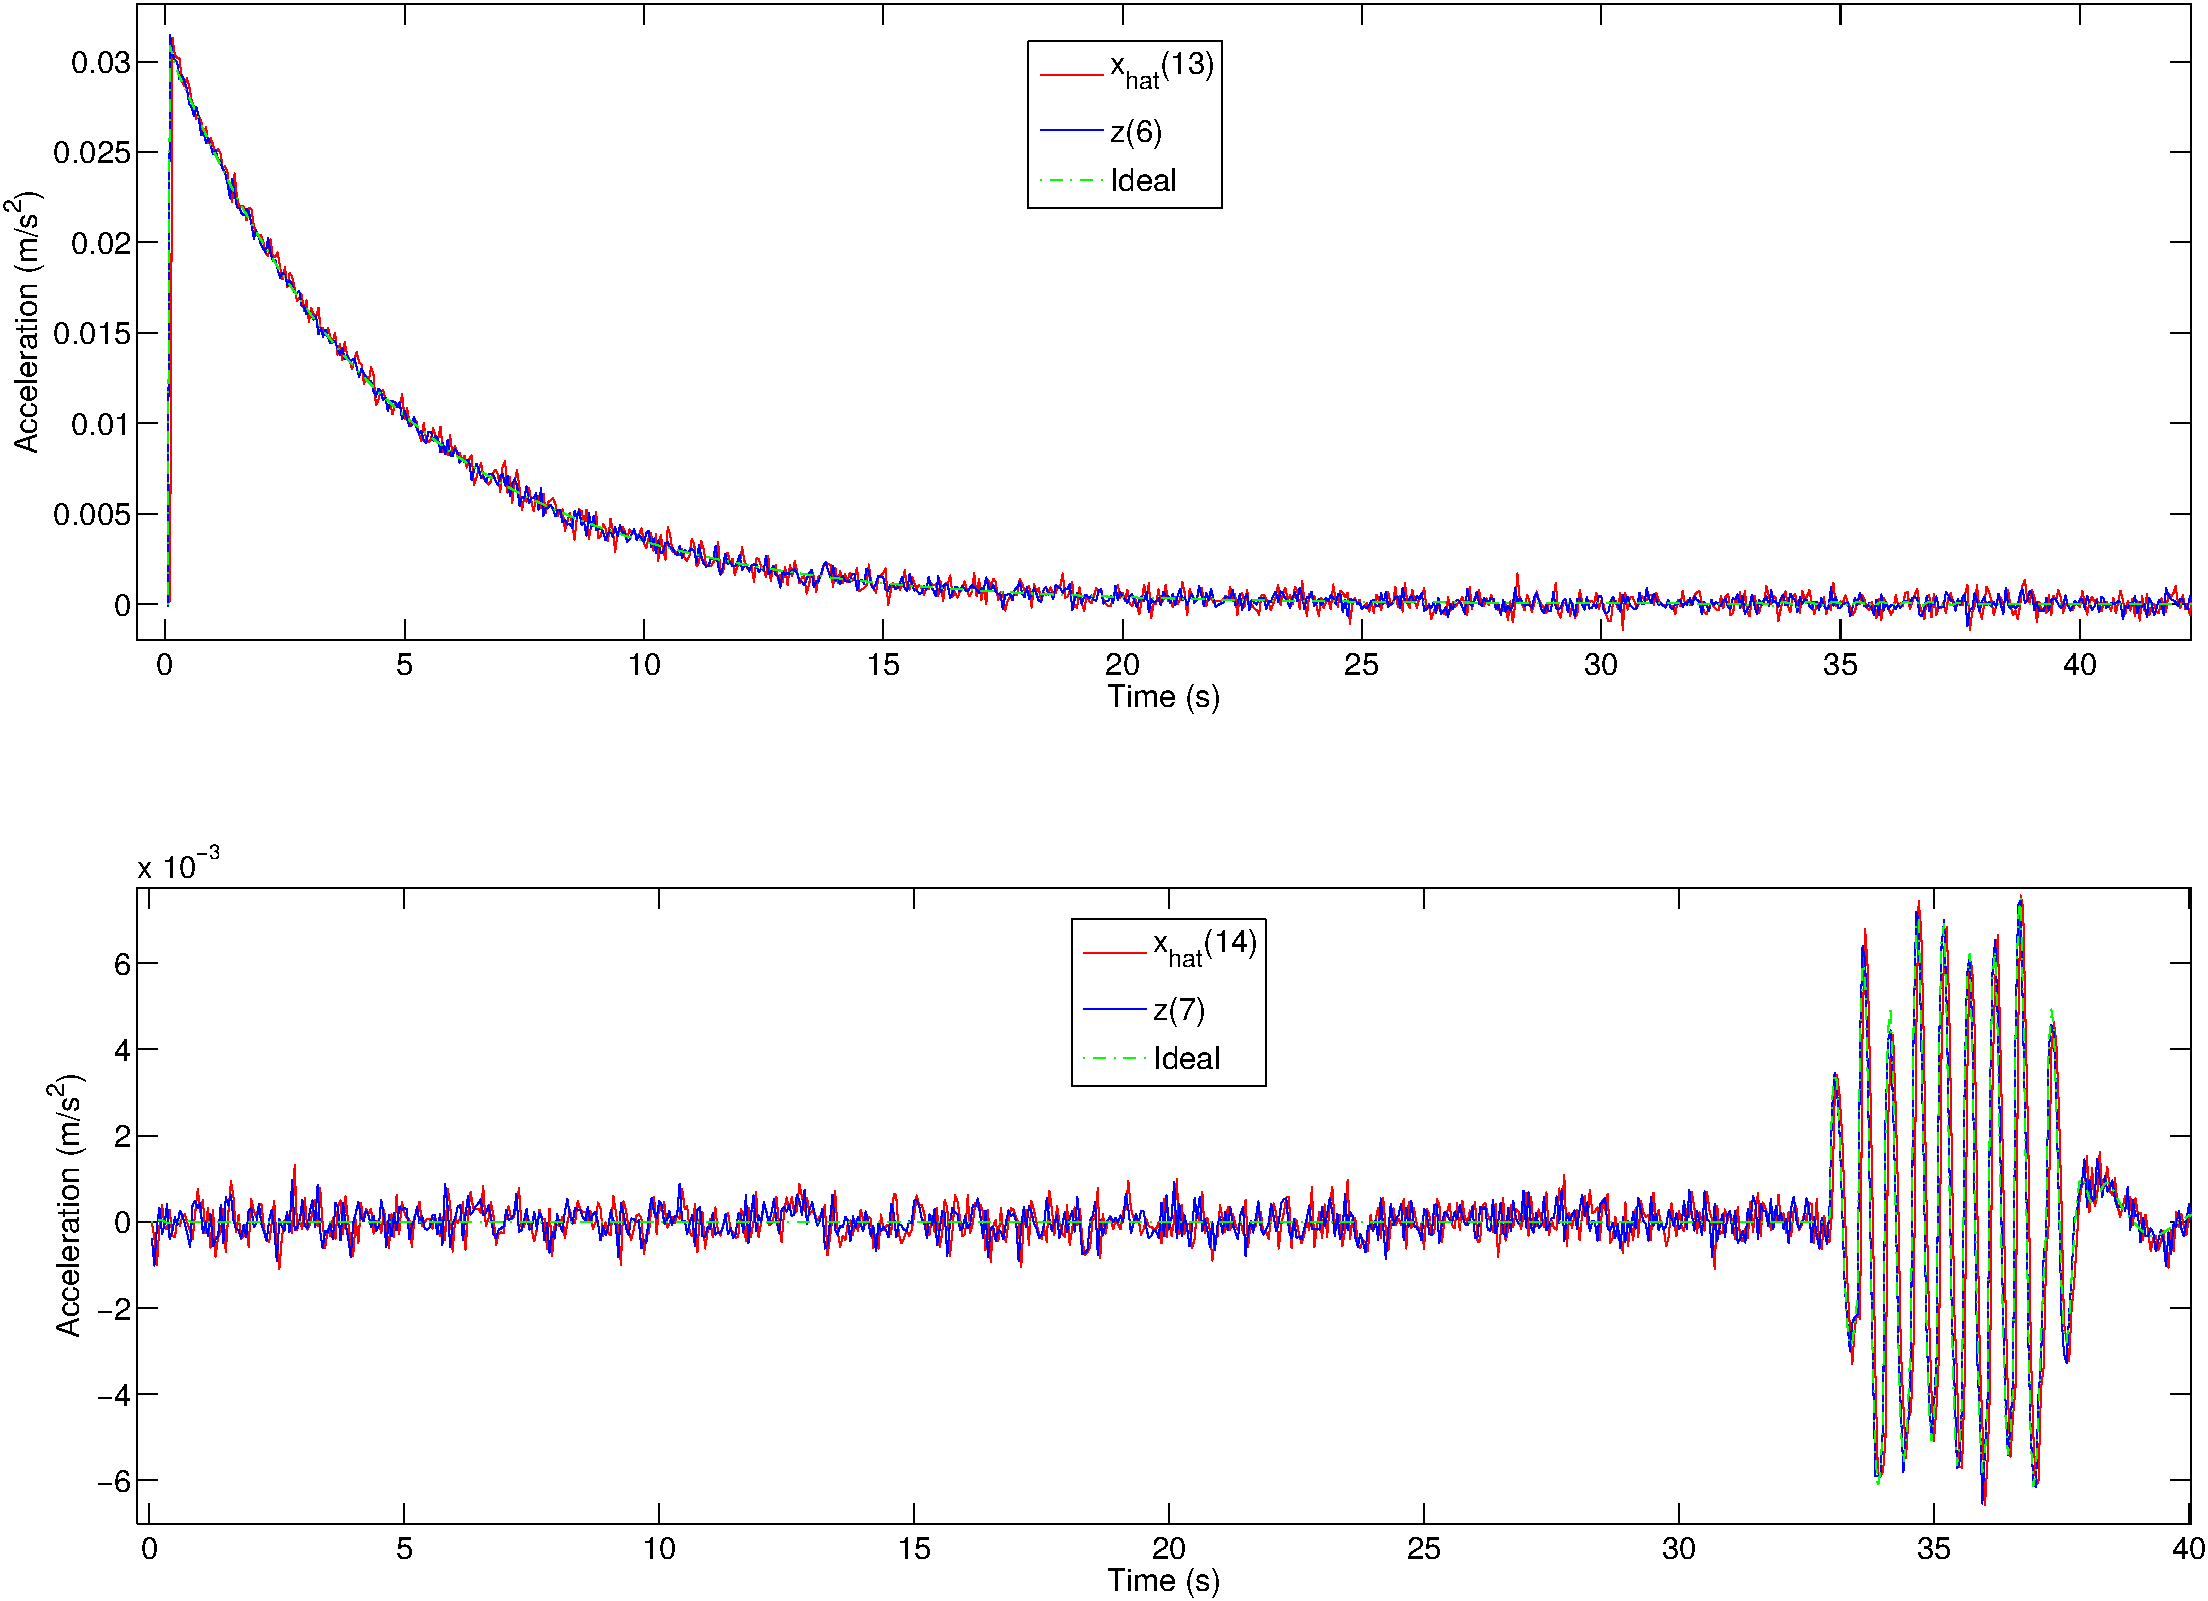
\includegraphics[width=0.9\textwidth]{../../code/matlab/accel0,00001}
  \caption{Measurement and estimate of acceleration in surge and sway.}
  \label{fig:uvacceltest}
\end{figure}
Afterwards is the velocity of the AAUSHIP tuned. This is done in the same manor, where the velocity of a step function needs to look like on figure \ref{fig:uvtest}.
\begin{figure}
  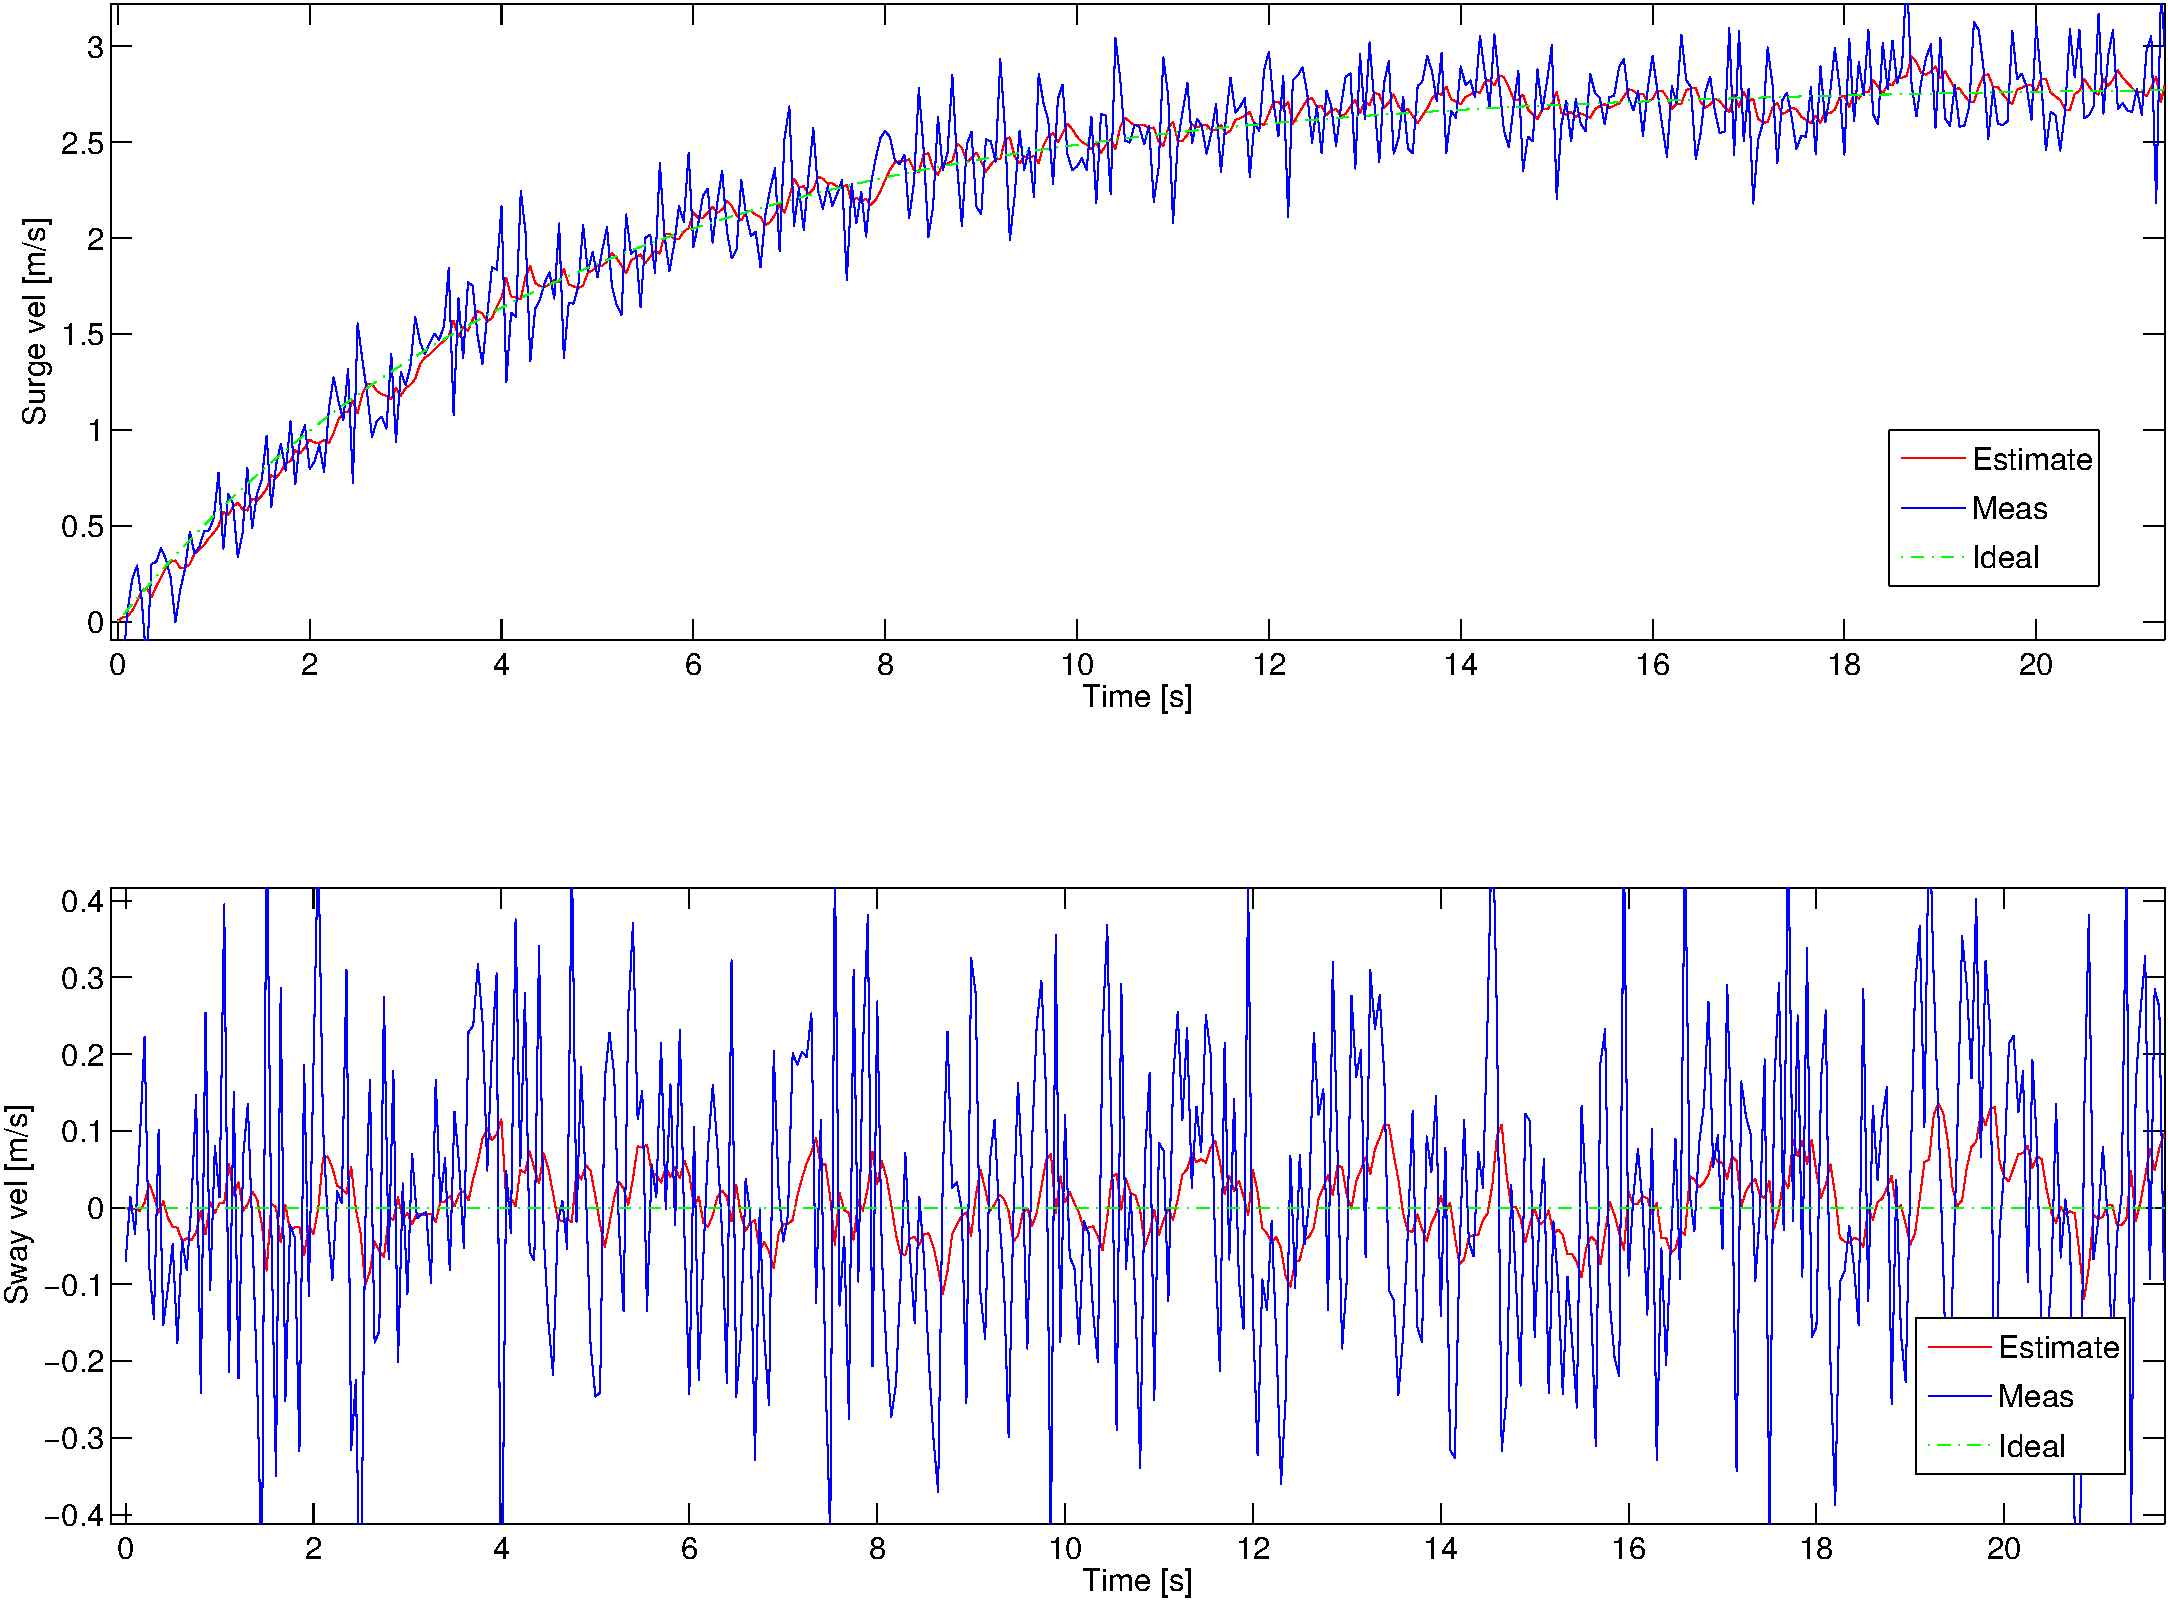
\includegraphics[width=0.9\textwidth]{../../code/matlab/uv0,00001}
  \caption{Measurement and estimate of velocity in surge and sway.}
  \label{fig:uvtest}
\end{figure}
At last is the position tuned, which is the one with largest relative noise from the measurements. This forces the value in Q to be smaller thus making the AAUSHIP trust the model prediction more than then measurements. A position plot with two different values in Q can be seen on figure \ref{fig:postest0,00001}.
\begin{figure}
\centering
  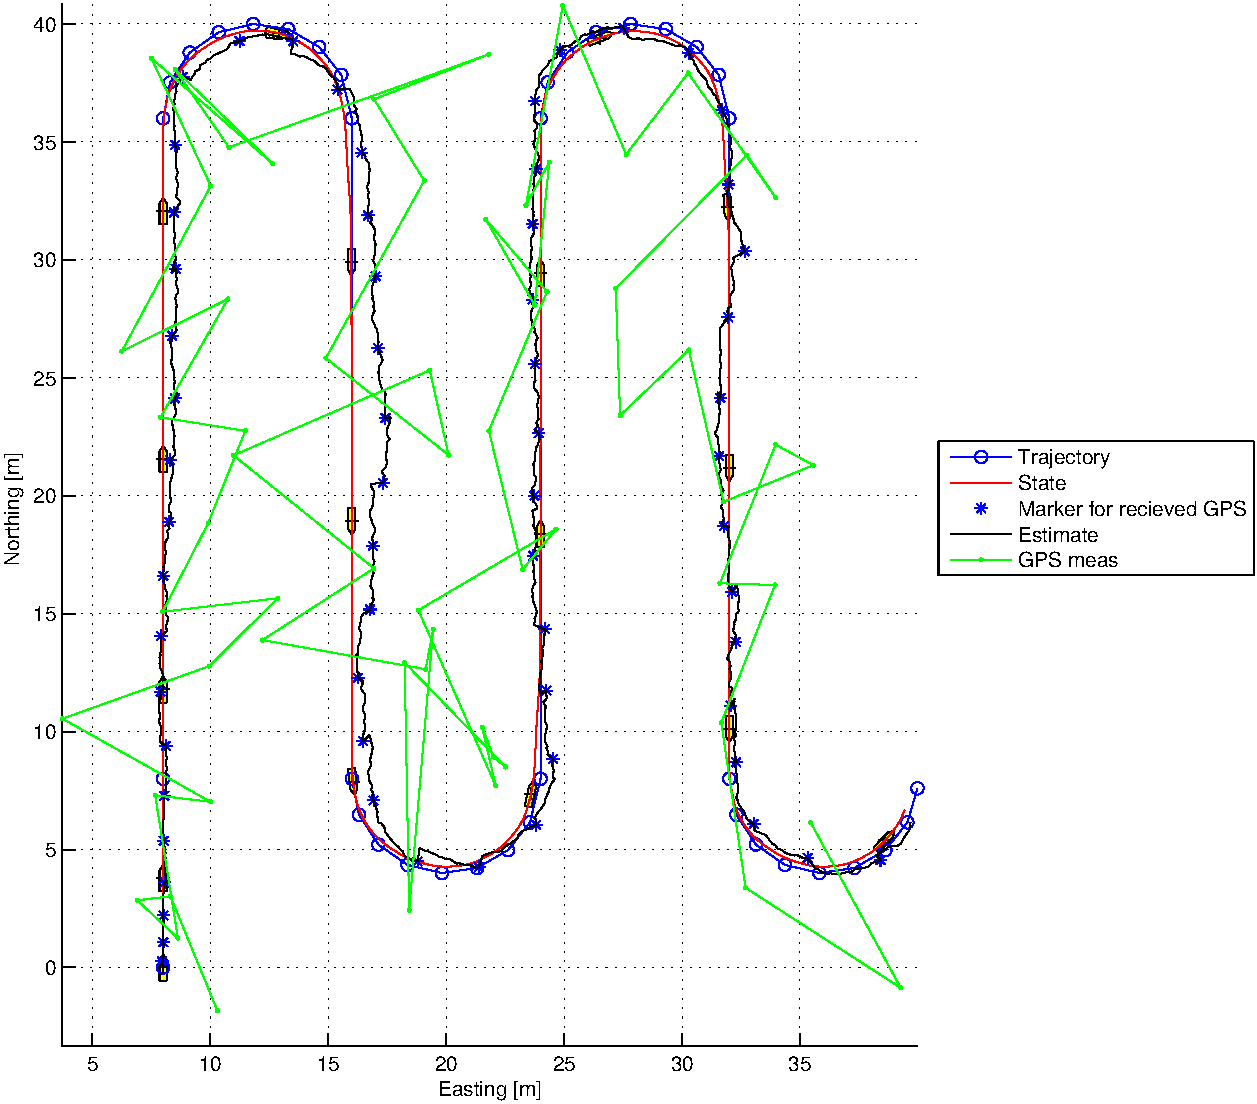
\includegraphics[width=0.8\textwidth]{../../code/matlab/q0,001}
  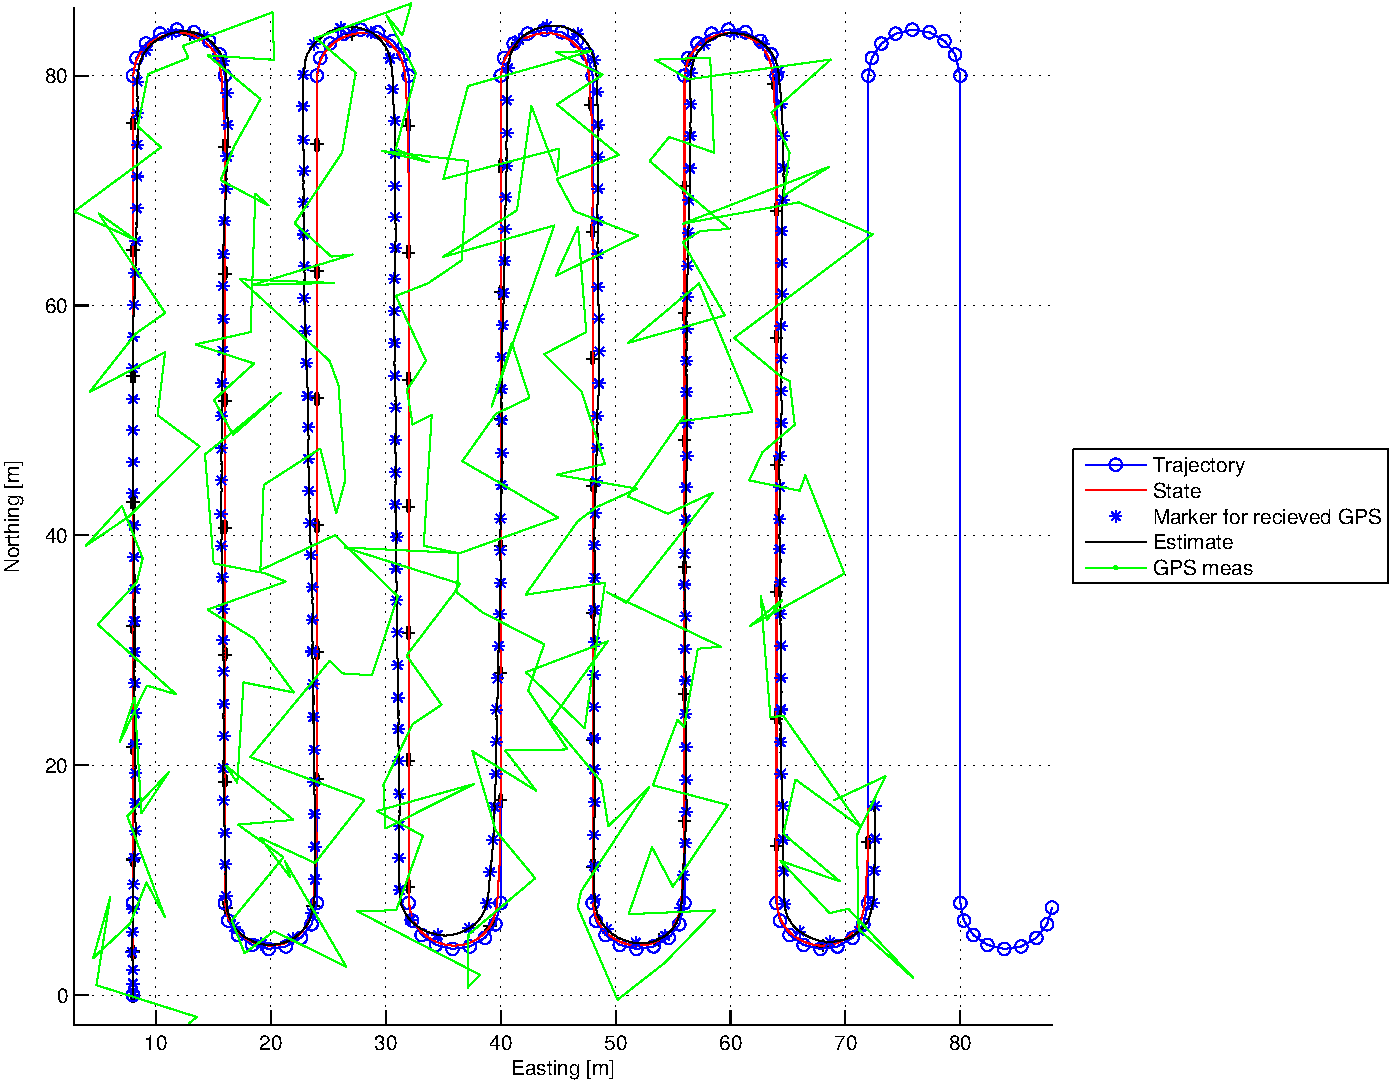
\includegraphics[width=0.8\textwidth]{../../code/matlab/q0,00001}
  \caption{Simulated and filtered measurements of AAUSHIP tracking a trajectory. First figure is with low sensor variance of the NED measurement, and second figure is with high sensor variance of the NED measurement.}
  \label{fig:postest0,00001}
\end{figure}
The one with the lowest value in Q gives the best position fit of these, which also follows the intuition of how the \ac{KF} should work. The resulting Q matrix is tuned to be
\begin{alignat*}{5}
&Q_k = \diag{\mathbf{w}} \text{, where} \\ \nonumber
&\sigma_{N}^2 = 0.001,\quad& &\sigma_{E}^2 = 0.001,\quad& &\sigma_{x_{b}}^2 = 0.001,\quad& &\sigma_{y_{b}}^2 = 0.001,\\ \nonumber
&\sigma_{\phi}^2 = 0.01,\quad& &\sigma_{\theta}^2 = 0.01,\quad& &\sigma_{\psi}^2 = 0.000001,\\ \nonumber
&\sigma_{u}^2 = 0.01,\quad& &\sigma_{v}^2 = 0.01,\quad& &\sigma_{p}^2 = 0.001,\quad& &\sigma_{q}^2 = 0.001,\quad& &\sigma_{r}^2 = 0.001,\\ \nonumber
&\sigma_{\dot u}^2 = 0.01,\quad& &\sigma_{\dot v}^2 = 0.01,\quad& &\sigma_{\dot p}^2 = 0.01,\quad& &\sigma_{\dot q}^2 = 0.01,\quad& &\sigma_{\dot r}^2 = 0.01
\end{alignat*}

\subsection{GPS in the Closed Loop}
The precision of the normal \ac{GPS} receiver is some times bigger than the desired resolution of the measurement resolution. The means that has been chosen to resolve this problem, is to use a kind of absolute positioning system which has better performance in this respect. A solution to his is the \ac{RTK}\ \ac{GPS} which can achieve way better positioning precision. This system uses a technique with a base station and a rovering device to correct for disturbances present in the local working area, such as atmospheric phenomena that can disturb the receiver. This system requires a direct data connection between the base station and the device on the rover \citep{rtk}.

Some experiments with this setup has been performed by the authors
using RTKLIB and LEA-4T receivers, but this has proven to be
problematic as soon as the rover is moving. This is kind of a do it
yourself way of getting a \ac{RTK} system. Commercial systems do exist
that work better, but these are fairly expensive to acquire. Therefore
it has been decided to make the system such that is will work with a
standard \ac{GPS} module, and optionally use \ac{RTK} with logging,
where it is possible to post process the data to get the exact
positions of where the ships has actually sailed. \todo{Er dette stadig sådan vi gør det? Jeppe}

This can be done, because the lawnmower reference trajectory the ships
shall follow is not a hard requirement from the mapping point of view,
they are only intended to distribute the scanning area such that it is
scanned fairly even. The reference trajectory generation is described
in chapter~\vref{ch:pathgen}. The ship is also pitching an rolling,
which cannot be controlled, and hence it makes no sense to make the
ship positioning overly accurate. This is seen from the perspective
that the ships main task is to cover the seabed with measurements,
thus it is only important to know the actual position and attitude of
the ship. This can be logged from the \ac{RTK} \ac{GPS} and then used
to determine the actual position and therefore the actual measurement
point of the seabed can be calculated.

\subsection{In Absence of \ac{GPS} Signal}
When there is no \ac{GPS} signal it is not possible to make any new estimates based from the measurements. This results in a model based phase of the controlling of the AAUSHIP. Therefore the AAUSHIP needs to converge to the predetermined trajectory based on how the model of the ship would do it. When a new \ac{GPS} signal is present this needs to be taken into account and thereby used as a correction to the model prediction. When the signal is absent there are different ways to handle this in the model. One of the ways is to set the variance of the sensor noise from the \ac{GPS} high. This value could be around $10 \cdot 10^9$ to ensure that the model does not take the measurement from the \ac{GPS} into account.

\subsection{Sample Rates}
If the different sensor measurements are not sampled with the same rate will the lower sample rates be untrue. This induces the same situation as if the \ac{GPS} signal is absent, thus setting the variances of these measurements high. The same situation will occur as with the missing \ac{GPS} signal, making the measurement be highly untrusted and only taking in the model prediction for that particular sample.

\subsection{Overall filter test and conclusion}
\todo{Der skal her samles op på filteret som er imp i matlab}

\section{Addition to the \acl{KF}}
The heading reference can be estimated both from the \ac{GPS} measurements and the from the \ac{IMU} measurements. The simulation model is using the measurement from one \ac{GPS}, due to the implementation of the single \ac{GPS}. The noise have been measured from the \ac{GPS} thus setting the accuracy based on this. When the \ac{RTK} \ac{GPS} will become implemented this can lower the noise variance from the measurements by fusing the two \ac{GPS}s. The measurements from the \ac{IMU} can too be used to estimate the attitude and the heading. All of these sensor measurements can be fused together in the \ac{KF}, such that the two \ac{GPS}s can give an estimate of the heading and include the \ac{IMU}. The \ac{GPS}s will also be used to estimate the \ac{SOG} together. When the \ac{RTK} \ac{GPS} is expected to have a lower variance both in position and \ac{SOG} measurements thus making the fusion of this preferable and resulting in a better estimate of both position and \ac{SOG}. Since the variance from the normal \ac{GPS} seems relatively high, it is expected that the main \ac{GPS} will be the \ac{RTK} \ac{GPS}.



%"Det lange af det korte er" - LOL, sagt af en buisness mand i toget, han meste lidt det modsatte. Selvom samtalen faktisk blev rimelig lang :p #FolkFraÅrhus
